\documentclass[border=1px]{standalone}
\usepackage{tikz}
\usetikzlibrary{positioning}
\begin{document}
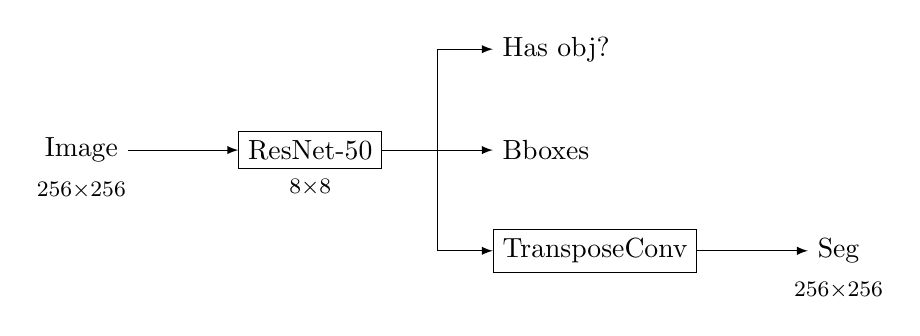
\begin{tikzpicture}[node distance=5ex and 4em]
\node (image) {Image};
\node [below=0pt of image, font=\footnotesize] {$256{\times}256$};
\node [draw, right=of image] (model) {ResNet-50};
\node [below=0pt of model, font=\footnotesize] {$8{\times}8$};
\node [above right=of model] (hasobj) {Has obj?};
\node [right=of model] (bboxes) {Bboxes};
\node [draw, below right=of model] (tconv) {TransposeConv};
\node [right=of tconv] (seg) {Seg};
\node [below=0pt of seg, font=\footnotesize] {$256{\times}256$};

\draw[-latex] (image) -- (model);
\draw[-latex] (model.east) ++(2em,0) |- (hasobj);
\draw[-latex] (model) -- (bboxes);
\draw[-latex] (model.east) ++(2em,0) |- (tconv);
\draw[-latex] (tconv) -- (seg);
\end{tikzpicture}
\end{document}

